%%%%%%%%%%%%%%%%%%%%%%%%%%%%%%%%%%%%%%%%%
% Structured General Purpose Assignment
% LaTeX Template
%
% This template has been downloaded from:
% http://www.latextemplates.com
%
% Original author:
% Ted Pavlic (http://www.tedpavlic.com)
%
% Note:
% The \lipsum[#] commands throughout this template generate dummy text
% to fill the template out. These commands should all be removed when 
% writing assignment content.
%
%%%%%%%%%%%%%%%%%%%%%%%%%%%%%%%%%%%%%%%%%

%----------------------------------------------------------------------------------------
%	PACKAGES AND OTHER DOCUMENT CONFIGURATIONS
%----------------------------------------------------------------------------------------

\documentclass{cctart}

\usepackage{multirow}
\usepackage{amssymb}

\usepackage{fancyhdr} % Required for custom headers
\usepackage{lastpage} % Required to determine the last page for the footer
\usepackage{extramarks} % Required for headers and footers
\usepackage{graphicx} % Required to insert images
\usepackage{lipsum} % Used for inserting dummy 'Lorem ipsum' text into the template

% Margins
\topmargin=-0.45in
\evensidemargin=0in
\oddsidemargin=0in
\textwidth=6.5in
\textheight=9.0in
\headsep=0.25in 

\linespread{1.1} % Line spacing

% Set up the header and footer
\pagestyle{fancy}
\lhead{\hmwkAuthorName} % Top left header
\chead{\hmwkClass\ : \hmwkTitle} % Top center header
\rhead{\firstxmark} % Top right header
\lfoot{\lastxmark} % Bottom left footer
\cfoot{} % Bottom center footer
\rfoot{Page\ \thepage\ of\ \pageref{LastPage}} % Bottom right footer
\renewcommand\headrulewidth{0.4pt} % Size of the header rule
\renewcommand\footrulewidth{0.4pt} % Size of the footer rule

\setlength\parindent{0pt} % Removes all indentation from paragraphs

%----------------------------------------------------------------------------------------
%	DOCUMENT STRUCTURE COMMANDS
%	Skip this unless you know what you're doing
%----------------------------------------------------------------------------------------

% Header and footer for when a page split occurs within a problem environment
\newcommand{\enterProblemHeader}[1]{
\nobreak\extramarks{#1}{#1 continued on next page\ldots}\nobreak
\nobreak\extramarks{#1 (continued)}{#1 continued on next page\ldots}\nobreak
}

% Header and footer for when a page split occurs between problem environments
\newcommand{\exitProblemHeader}[1]{
\nobreak\extramarks{#1 (continued)}{#1 continued on next page\ldots}\nobreak
\nobreak\extramarks{#1}{}\nobreak
}

\setcounter{secnumdepth}{0} % Removes default section numbers
\newcounter{homeworkProblemCounter} % Creates a counter to keep track of the number of problems

\newcommand{\homeworkProblemName}{}
\newenvironment{homeworkProblem}[1][Problem \arabic{homeworkProblemCounter}]{ % Makes a new environment called homeworkProblem which takes 1 argument (custom name) but the default is "Problem #"
\stepcounter{homeworkProblemCounter} % Increase counter for number of problems
\renewcommand{\homeworkProblemName}{#1} % Assign \homeworkProblemName the name of the problem
\section{\homeworkProblemName} % Make a section in the document with the custom problem count
\enterProblemHeader{\homeworkProblemName} % Header and footer within the environment
}{
\exitProblemHeader{\homeworkProblemName} % Header and footer after the environment
}

\newcommand{\problemAnswer}[1]{ % Defines the problem answer command with the content as the only argument
\noindent\framebox[\columnwidth][c]{\begin{minipage}{0.98\columnwidth}#1\end{minipage}} % Makes the box around the problem answer and puts the content inside
}

\newcommand{\homeworkSectionName}{}
\newenvironment{homeworkSection}[1]{ % New environment for sections within homework problems, takes 1 argument - the name of the section
\renewcommand{\homeworkSectionName}{#1} % Assign \homeworkSectionName to the name of the section from the environment argument
\subsection{\homeworkSectionName} % Make a subsection with the custom name of the subsection
\enterProblemHeader{\homeworkProblemName\ [\homeworkSectionName]} % Header and footer within the environment
}{
\enterProblemHeader{\homeworkProblemName} % Header and footer after the environment
}
   
%----------------------------------------------------------------------------------------
%	NAME AND CLASS SECTION
%----------------------------------------------------------------------------------------

\newcommand{\hmwkTitle}{Assignment\ \#1} % Assignment title
\newcommand{\hmwkDueDate}{March\ 1,\ 2016} % Due date
\newcommand{\hmwkClass}{Algorithms} % Course/class
\newcommand{\hmwkAuthorName}{Zhaoyang Li (2014013432)} % Your name

%----------------------------------------------------------------------------------------
%	TITLE PAGE
%----------------------------------------------------------------------------------------

\title{
\vspace{2in}
\textmd{\textbf{\hmwkClass:\ \hmwkTitle}}\\
\normalsize\vspace{0.1in}\small{Due\ on\ \hmwkDueDate}\\
\vspace{3in}
}

\author{\textbf{\hmwkAuthorName}}
\date{} % Insert date here if you want it to appear below your name

%----------------------------------------------------------------------------------------

\begin{document}

\maketitle

%----------------------------------------------------------------------------------------
%	TABLE OF CONTENTS
%----------------------------------------------------------------------------------------

%\setcounter{tocdepth}{1} % Uncomment this line if you don't want subsections listed in the ToC

\newpage
\tableofcontents
\newpage

%----------------------------------------------------------------------------------------
%	PROBLEM 1
%----------------------------------------------------------------------------------------

\begin{homeworkProblem}
\begin{homeworkSection}{(1)} % Section within problem
Prove that $2n+\Theta(n^2)=\Theta(n^2)$.

\problemAnswer{ % Answer
Proof:

Let $f(n)=\Theta(n^2)$. By definition, there exists positive constants $c_1, c_2$ such that
$$c_1n^2 \leq f(n)\leq c_2n^2$$
Let $g(n) = f(n) + 2n$. We have
$$c_1n^2 + 2n \leq g(n) \leq c_2n^2 + 2n$$
For all $n>\frac{2}{c_2}$, $2n<c_2n^2$. $c_2n^2 + 2n < 2c_2n^2$. Meanwhile, $c_1n^2 + 2n > c_1n^2$,
$$c_1n^2 \leq g(n) \leq 2c_2n^2 $$
Choosing $c_1'=c_1, c_2'=2c_2$, by definition we have $g(n)=\Theta(n^2)$. QED.
}
\end{homeworkSection}

%--------------------------------------------
\begin{homeworkSection}{(2)} % Section within problem
Prove that $\Theta(g(n))\cup o(g(n))=\emptyset$.

\problemAnswer{ % Answer
Proof:

Assume that there exists an $f$ such that $f(n) \in \Theta(g(n))\cup o(g(n))$.

Since $f(n) \in \Theta(g(n))$, there exists positive constants $c_1, c_2, n_0$ such that for all $n>n_0$, 

$$c_1g(n)\leq f(n) \leq c_2g(n)$$

Since $f(n) \in o(g(n))$, for all $c>0$, there exists $n_1>0$, such that for all $n>n_1$, $0\leq f(n) < cg(n)$. Let $c$ be $c_1$, we have

$$f(n) < c_1g(n)$$

Let $n_2=\max{(n_0, n_1)}$. For all $n>n_2$, we have both $f(n) < c_1g(n)$ and $f(n) \geq c_1g(n)$ in contradiction.

So $\Theta(g(n))\cup o(g(n))=\emptyset$. QED.
}
\end{homeworkSection}

%--------------------------------------------
\begin{homeworkSection}{(3)} % Section within problem
Prove that $\Theta(g(n))\cap o(g(n))\neq O(g(n))$.

\problemAnswer{ % Answer
Proof:

Let $g(n)=n^2$, $f(n)=n^(1+\sin n)$. For all $n>0$, $0<f(n)\leq g(n)$, so $f(n) \in O(g(n))$.

However, $\forall k \in \mathbb{N}^*, f(k\pi + \frac{3}{2}\pi)=0$. Thus, there does not exist such $c>0$ that $\forall n>n_0, cn^2<f(n)$, meaning that $f(n) \notin \Theta(g(n))$.

Meanwhile, $\forall n=k\pi + \frac{1}{2}\pi (k \in \mathbb{N}^*), f(n)=g(n)$. Thus, $\forall n_0>0$, there exists $n$ s.t. $f(n)=g(n)$. Thus, $f(n) \notin o(g(n))$.

QED.
}

\end{homeworkSection}

%--------------------------------------------
\begin{homeworkSection}{(4)} % Section within problem
Prove that $\max((f(n),g(n)))=\Theta(f(n)+g(n))$.

\problemAnswer{ % Answer
Proof:

Let $h(n)=\max((f(n),g(n)))$. 

$$\frac{1}{2} (f(n)+g(n))\leq h(n) \leq f(n)+g(n)$$

Choosing $c_1=\frac{1}{2}, c_2=1$, by definition we have $h(n)=\Theta(f(n)+g(n))$. QED.
}
\end{homeworkSection}

%--------------------------------------------
\begin{homeworkSection}{(5)} % Section within problem
Solve the recurrence $T(n) = 2T(\sqrt{n}) + 1$.

\problemAnswer{ % Answer
Let $m=\log n$, then $T(2^m) = 2 T(2^\frac{m}{2}) + 1$.

Let $S(m) = T(2^m)$, then $S(m) = 2 S(\frac{m}{2}) + 1$.

We have $a=2, b=2, F(m)=m^0$, and we have that $m^{\log_ba}=m^1$. 

Since $m^1$ is polynomially larger than $m$, applying case 1 in the Master Theorem, 

$$S(m)=\Theta(m^2)$$

Thus, 

$$T(n)=\Theta(\log^2 n)$$

QED.
}
\end{homeworkSection}

%--------------------------------------------
\begin{homeworkSection}{(6)} % Section within problem
Solve the recurrence $nT(n) = (n-2)T(n-1) + 2$.

\problemAnswer{ % Answer
Multiply by $(n-1)$,

$$n(n-1)T(n) = (n-1)(n-2)T(n-1) + 2(n-1)$$

Let $g(n) = n(n-1)T(n)$. Thus,

$$ g(n) = g(n-1) + 2(n-1)$$

$$g(n) = \sum_{i=1}^n 2(n-1) + g(1) = n(n-1) + g(1)$$

$$T(n) = \frac{g(n)}{n(n-1)} = 1 + \frac{g(1)}{n(n-1)} = \Theta(1)$$

QED.
}
\end{homeworkSection}

\end{homeworkProblem}

%----------------------------------------------------------------------------------------
%	PROBLEM 2
%----------------------------------------------------------------------------------------

\begin{homeworkProblem}
Compare naive matrix multiplication and the Strassen's algorithm.

\problemAnswer{
Both implemented in an recursive way in C++. To be compiled with Visual Studio 2012.

For code and run-time screenshots, please refer to the attachments.

Results\footnote{on an Intel Core i5 4120U Processor, 4GB DDR3 Memory, Windows 10 Pro} are as follows:


\begin{center}

CPU Time Consumed (microseconds)


\begin{tabular}{rrr}
\hline
Size of matrix& Naive& Strassen's\\
\hline
1& 0& 0\\
2& 0& 100\\
4& 200& 300\\
8& 1500& 2000\\
16& 9600& 16100\\
32& 69600& 88500\\
64& 609200& 643500\\
128& 4418300& 4537000\\
256& 35934400& 30109700\\
\hline
\end{tabular}
\end{center}
Seems that the cross-over point is somewhere between 128 and 256.

A double-logarithmic chart visualizing the data above:
\begin{center}
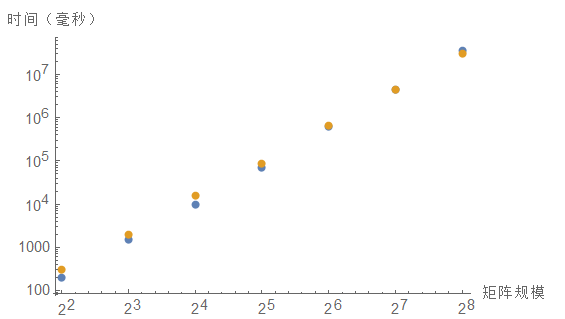
\includegraphics[width=0.75\columnwidth]{chart} 
\end{center}

Perfect linearity, verifying polynomial complexity. 

}

%--------------------------------------------


%--------------------------------------------

\end{homeworkProblem}



%----------------------------------------------------------------------------------------

\end{document}
